\section{EXPERIMENTS}
\subsection{Aerial Transformation}
In this experiment, we utilized a transformable hex-rotor with six-links. The whole weight is about 5.0[kg]. The three-dimensional position was tracked by a motion capture system, representing nearly ground truth, and sent to the onboard computer via Wi-Fi. The hardware platform is the same as that explained in Sec. IV. 
\par
We tested the stability of hovering of multilinks under a fixed form($\theta_1=\theta_2=\frac{\pi}{2}$, $\theta_3=0$, $\theta_4=\theta_5=-\frac{\pi}{2}$) and the result is shown in \figref{rotate_with_yaw}. In \figref{rotate_with_yaw}(a), each element of lifting force disperses after about 10[s], resulting that $u_3$(the third element of lifting force $\bm{u}$) reaches the upper limit(16.5[N]). The reason can be explained by the result shown in \figref{rotate_with_yaw}(b). After about 10[s], the error of yaw angle increases, and then a particular lifting force increases due to the feedback control of yaw angle. Normally, the error of yaw angle converges to the target angle  which is $0$ in this experiment  by the attitude control, however. Therefore, it is assumed that there are some factors which are not considered in the control model. As one of the factors, tilt of propeller axis resulting from the low rigidity of multilinks can be considered. If an propeller axis tilts, the moment around yaw axis is generated. The moment can be regarded as a disturbance which affects yaw angle. The moment generated by a propeller scales linearly with the lifting force generated by the propeller. This is written as:
\begin{equation}
  T_i=c_iF_i \ (i=1,\cdots,N)
\end{equation}
\begin{equation}
  c_i=\pm 0.01676
  \label{eq:coef_c}
\end{equation}
where $T_i$ and $F_i$ indicate the moment and lifting force generated by i-th propeller, respectively. Also note that $c_i$ is a constant rate between moment and force. The sign of $c_i$ is positive when the propeller rotates CCW and negative when the propeller rotates CW. In our multilinks, the value of $c_i$ is shown in \equref{coef_c}. That is to say, since the disturbance moment generated by tilt of the propeller is larger than the propeller moment($T_i$), resulting in divergence of the input vector $\bm{u}$. 
\par
Assuming this, we also performed a experiment on aerial transformation without the yaw control. The start and goal forms are as follows:
\begin{equation}
  \begin{cases}
    START: \theta_i = \frac{\pi}{3}\text{[rad]}\\
    GOAL: \theta_i = -\frac{\pi}{3}\text{[rad]}
  \end{cases}
\end{equation} 
\figref{hydrus_transformation} shows the snapshots of the aerial transformation, while \figref{transform_result} shows the change of joint angle, yaw angle and three-dimensional position($x,y,z$). Although the yaw angle does not converge due to the lack of yaw control, the three-dimensional position follows the target value. Therefore, we conclude that the feasibility of the aerial transformation without yaw control was experimentally demonstrated.

\begin{figure}[th]
  \begin{center}
    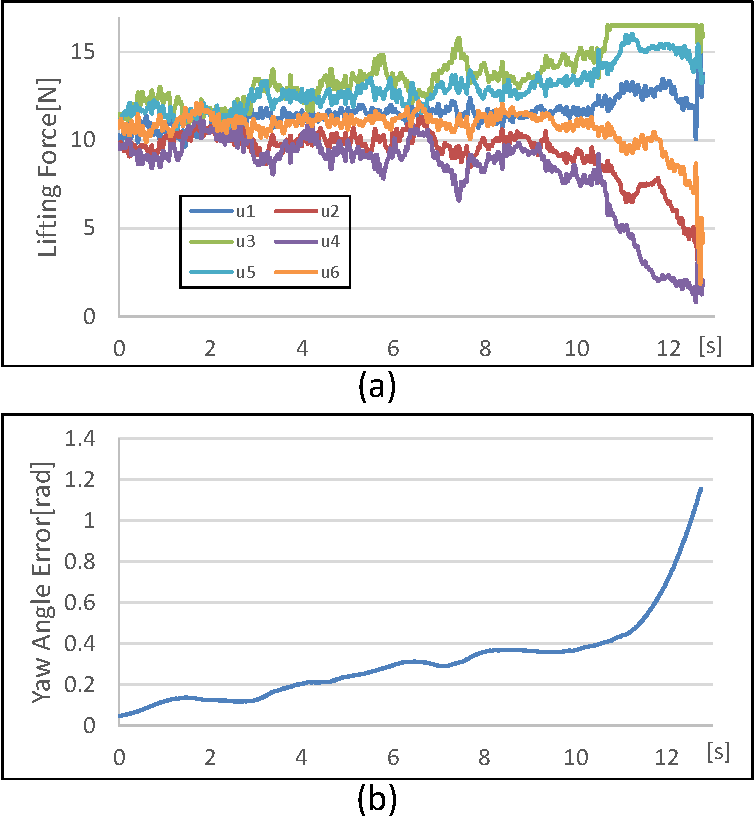
\includegraphics[width=1.0\columnwidth]{figs/rotate_with_yaw.pdf}
  \end{center}
  \caption{Experimental result of hovering under a fixed form with yaw control. (a): Change of lifting force generated by each propeller. (b): Change of yaw angle. \label{figure:rotate_with_yaw}}
\end{figure}

\begin{figure}[th]
  \begin{center}
    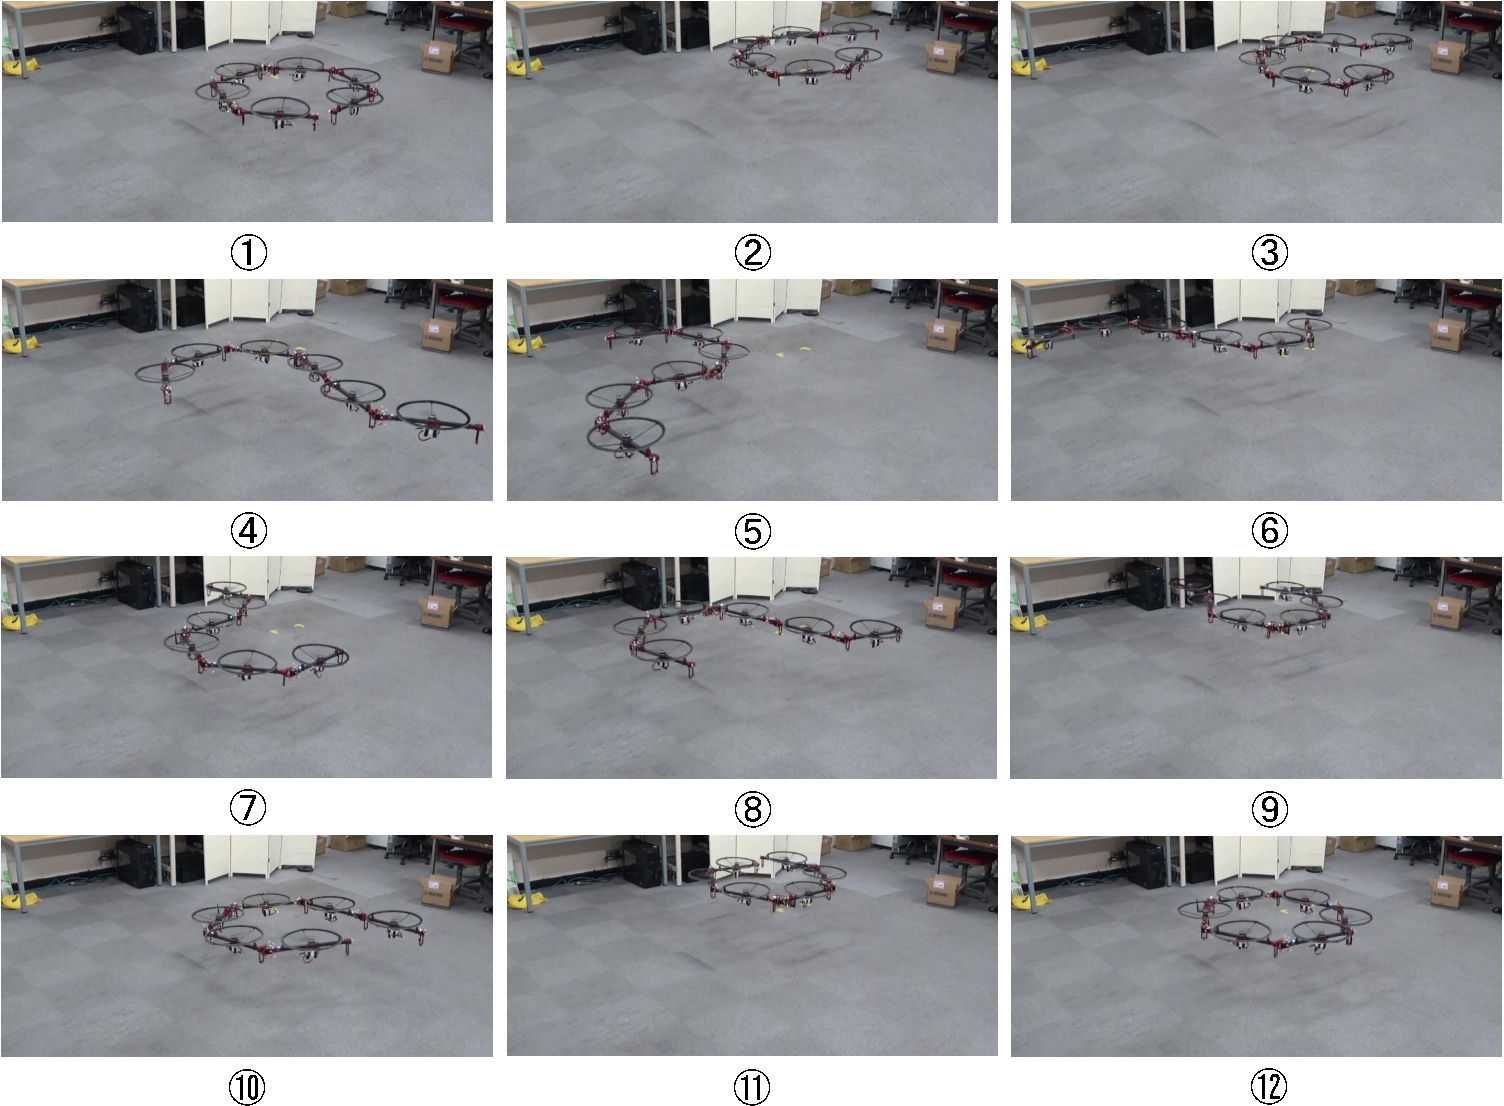
\includegraphics[width=1.0\columnwidth]{figs/hydrus_transformation.pdf}
  \end{center}
  \caption{Experiment of aerial transformation by six-links without yaw control: the start form is $(\theta_i=\frac{\pi}{3})$ and the goal form is $(\theta_i=-\frac{\pi}{3})$.\label{figure:hydrus_transformation}}
\end{figure}

\begin{figure}[th]
  \begin{center}
    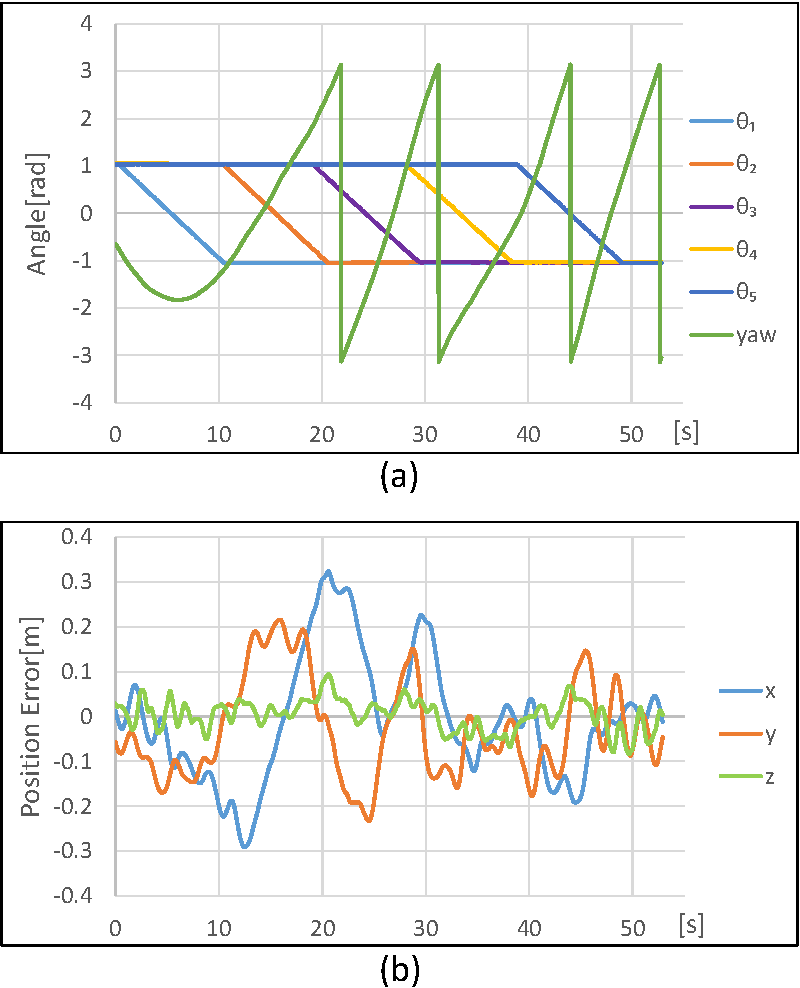
\includegraphics[width=0.9\columnwidth]{figs/transform_result.pdf}
  \end{center}
  \caption{(a): Change of angle of each joint and yaw angle. (b): Change of three-dimensional position error. \label{figure:transform_result}}
\end{figure}

\vspace{-0.5cm}
\subsection{Multiple Objects Transportation}
In this experiment, we utilized a transformable quad-rotor with four-links because of the limited experimental area. Also, the multilinks hovered without yaw controll due to the same reason as (a).  Also in this work, limiting target objects to ferrous objects, we construct an electromagnet gripper. The gripper comprises five electromagnets whose diameter is 20[mm] and four micro switches. Contact with an object can be detected by the signal of micro switches. The electromagnets are driven only while any switch is turned on to save the energy of batteries and to avoid the overheating of electromagnets. The gripper communicates with a computer by using USB-Serial.
\par
The number of target objects was set to two. Then, using the form optimization method, we calculated optimal forms shown in \figref{quad_state}. The additional mass is 0.551[kg], the sum weight of the target object and the electromagnet gripper. The final values of $V(\bm{u})$ shown under each form, especially that of form (b), are large relatively. The cause is considered that the four-links lacks the degree of freedom of transformation due to the constraints described in Sec. V(b).

\begin{figure}[t]
  \begin{center}
    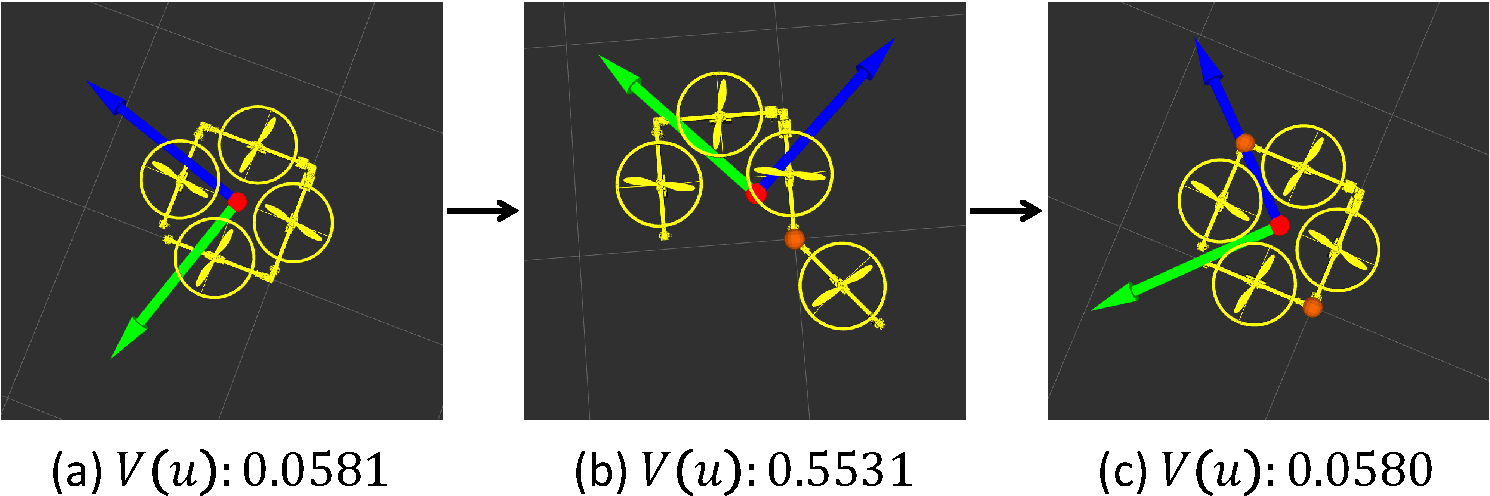
\includegraphics[width=1.0\columnwidth]{figs/quad_state.pdf}
  \end{center}
  \caption{The optimal forms of quad-rotor with four-links: the aerial robot grasps (a):no object (b): one object (c): two objects\label{figure:quad_state}}
\end{figure}

Then, we performed the experiment of multiple object transportation shown in \figref{experiment}. The process of multiple object transportation can be summarized as follows: $\textcircled{\scriptsize 1}$: approaching to the first object; $\textcircled{\scriptsize 2}\sim \textcircled{\scriptsize 4}$: grasping the first object and transforming to the optimal form(\figref{quad_state}(b)); $\textcircled{\scriptsize 5}$: approaching to the second object; $\textcircled{\scriptsize 6}\sim \textcircled{\scriptsize 8}$: grasping the second object and transforming to the optimal form(\figref{quad_state}(c)); $\textcircled{\scriptsize 9}\sim \textcircled{\scriptsize 10}$: approaching to and landing on the goal area. Note that the weight of the objects were given in advance and the optimal forms were calculated in off-line in this work. The positions of the objects were detected by a camera on the aerial robot with using HSV-Filter to detect the blue region. The images of the onboard camera is shown at lower left in \figref{experiment}. The detected object is surrounded by white contour in the images.
\if 0
\begin{figure}[H]
  \begin{center}
    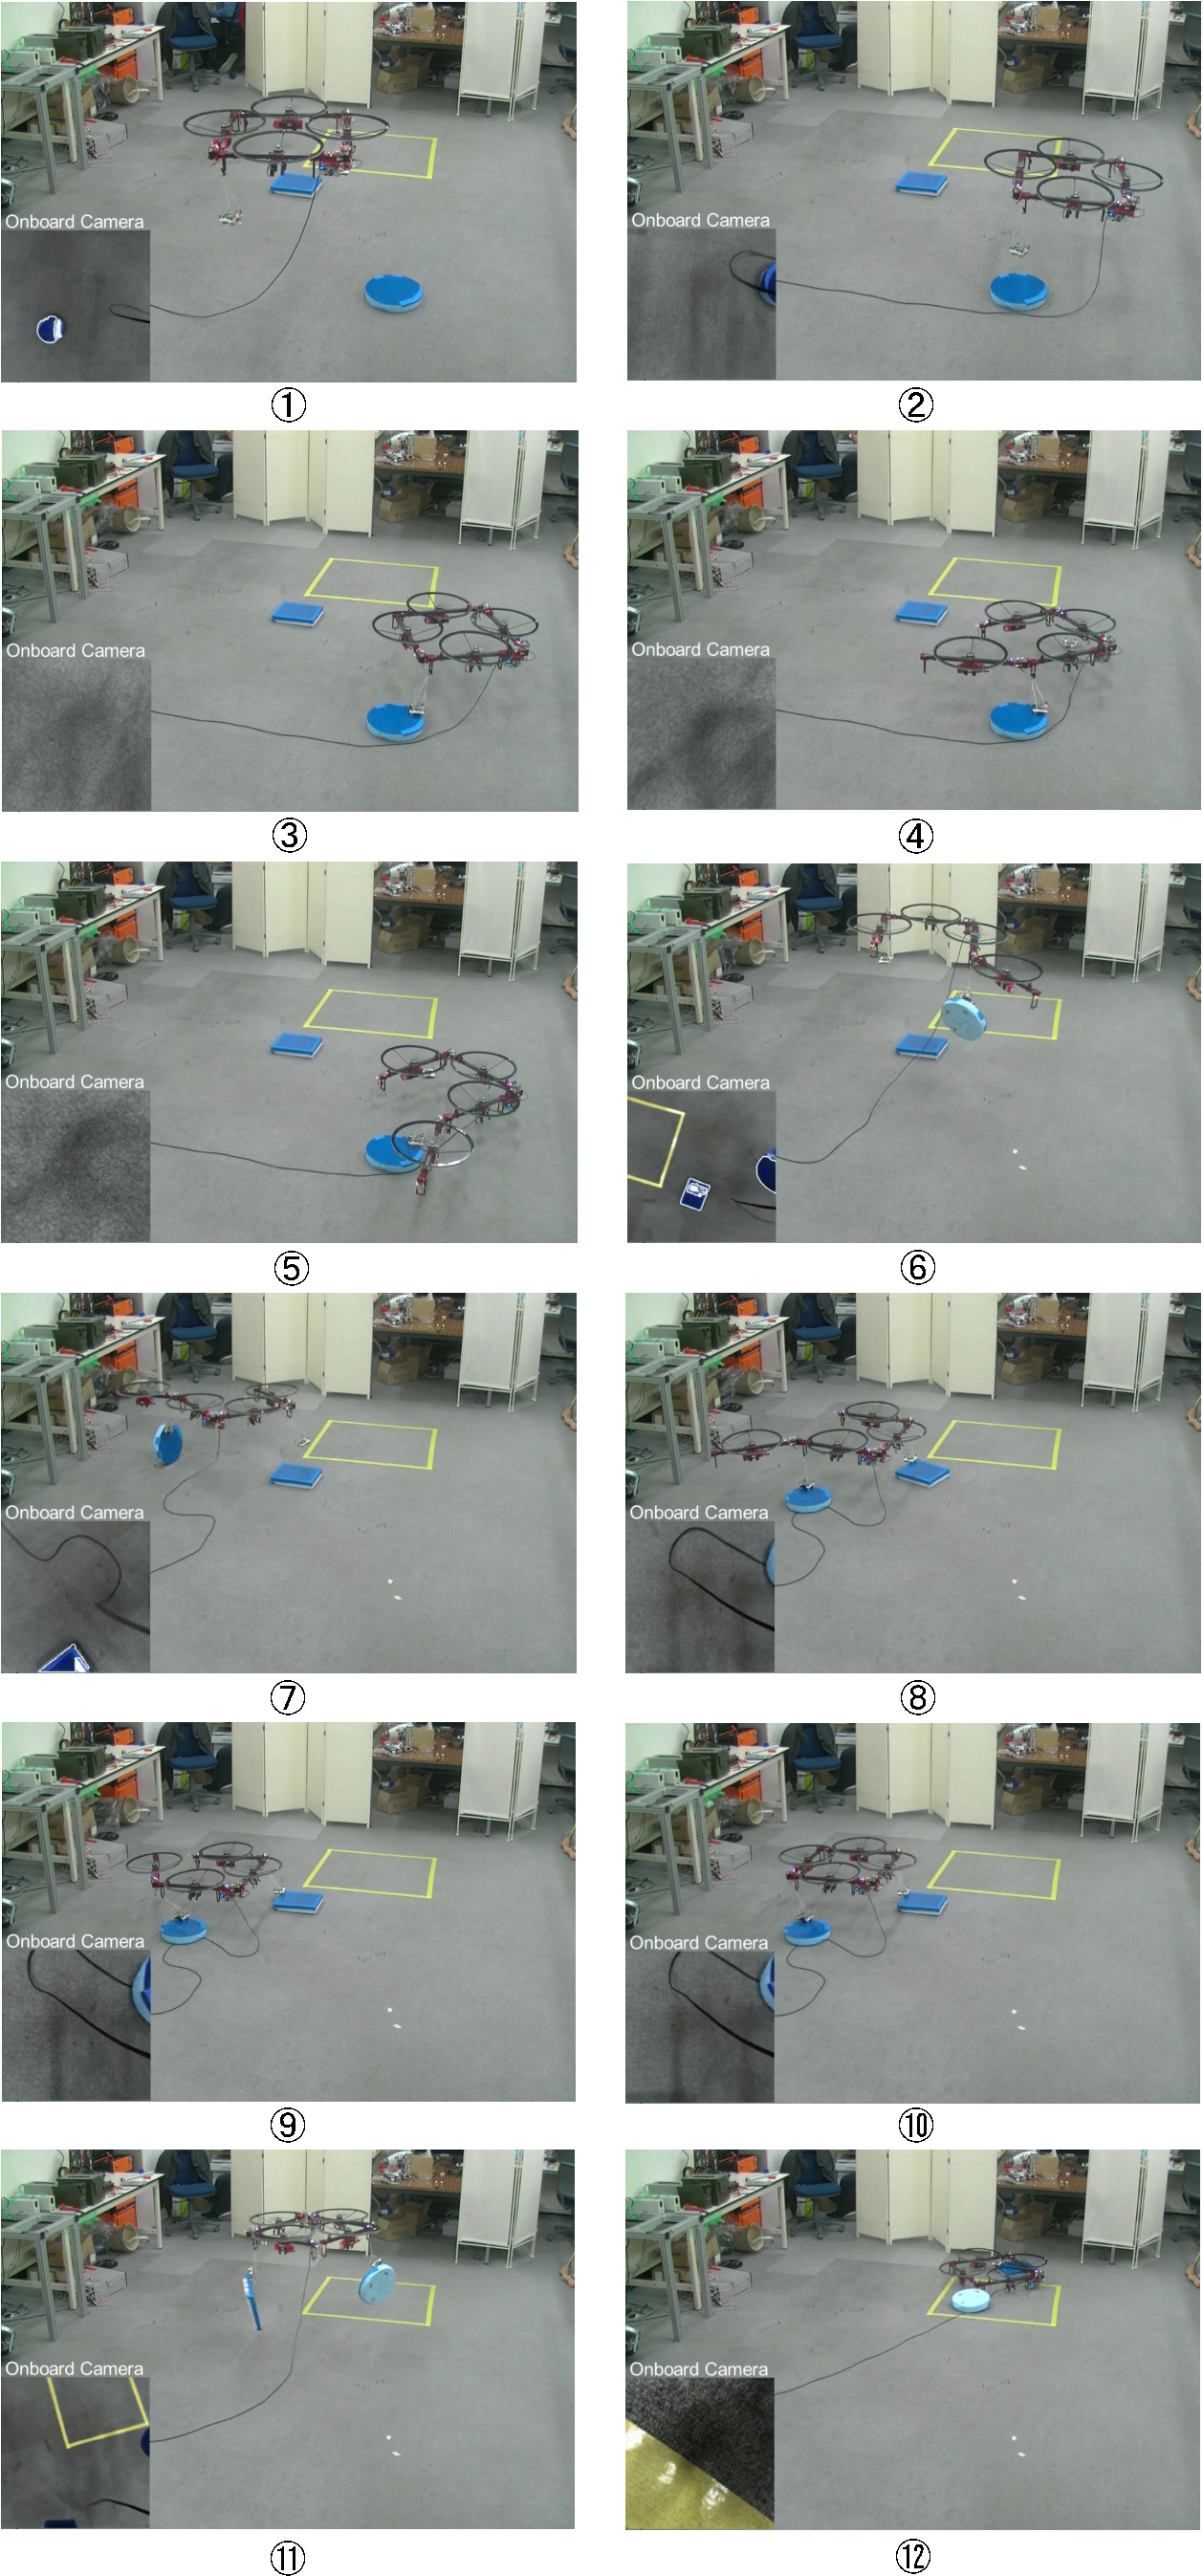
\includegraphics[width=1.0\columnwidth]{figs/experiment.pdf}
  \end{center}
  \caption{Experiment of multiple objects transportation: two ferrous objects are grasped and transported by the transformable aerial robot.\label{figure:experiment}}
\end{figure}
\fi
